\chapter*{Introduction}

In the aurora 2020-2021 for United States of America and maybe before, like 2019 for China, the world of High Performance Computing (HPC) will reach another milestone in the power of machines: the Exascale. 
These supercomputers will be $100$ times faster than the estimated overfall operations performed by the human brain and its $10^{16}$ \textbf{FL}oating point \textbf{O}perations \textbf{P}er \textbf{S}econd (FLOPS) and achieve a computational power of a trillion ($10^{18}$) FLOPS.
This odyssey started long time ago with the first vacuum tubes computers and the need of balistic computation in war. 
Nowdays the aim is very nearby and the power of a nation is represented by its army and money but also by the computational power of its supercomputers.
HPC's applications also spread into all the area of science and technology.\\

Since 1962, considering the Cray CDC 6600 as the first supercomputer, the power of those machines have increase following an observation of the co-fonder of the Intel company, Gordon Moore. 
Better known under the name of "Moore's Law", it speculates in 1965 that: considering the constant evoluation of technology the number of transistors on a dense integrated circuit will double approximately every two years. 
Thus, the computational power, that depend intrinsectly of the number of transistors on the chip, will increase and more important, as money is the sinews of war, the cost of the die for the same performances will decrease.  
This observation can be related to the supercomputers results through the years in the TOP500 list. 
As shown on figure~\ref{fig:intro_top500}, even if estimated in early 1965, the Moore's law seems to be accurate and sustainable. 

\begin{figure}
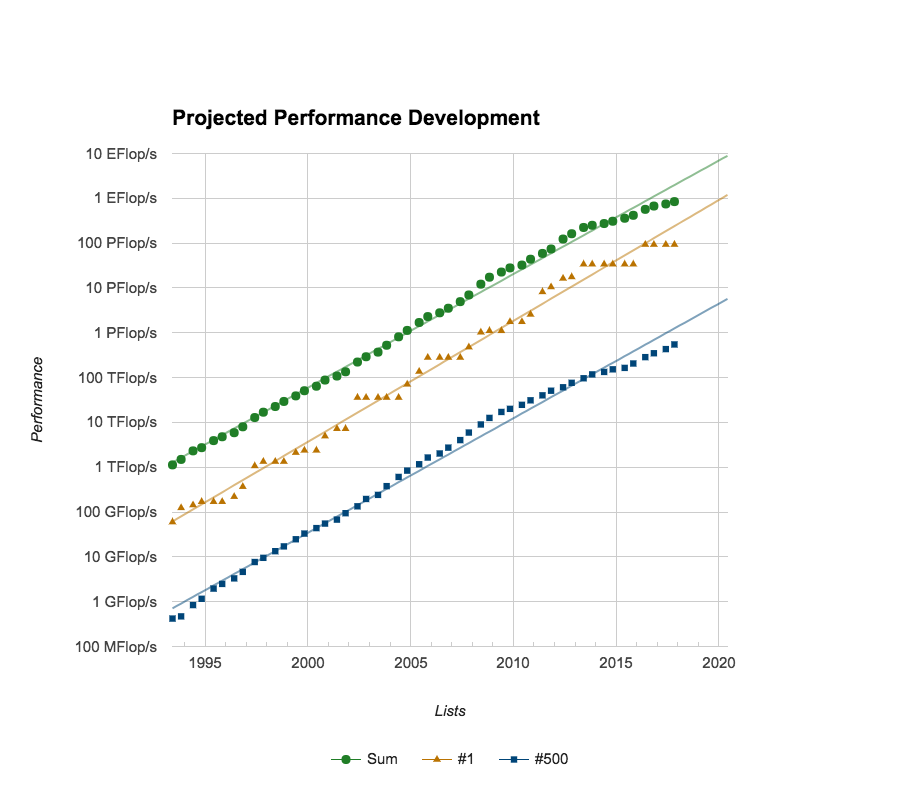
\includegraphics[width=\linewidth]{figures/introduction/top500_list_approximation.png}
\caption{Computational power evolution in the TOP500 list}
\label{fig:intro_top500}
\end{figure}

This linear evolution is not just gave by the shrink in the semiconductor with smaller transistors.
In fact the first one-core Central Processing Units (CPUs) were made using more transistors but also faster frequency.
But they faced limitations in reaching high frenquencies with the power consumption and the inherant cooling of the heat generated by the chip.
This is why, at some point in early twentieth century, IBM proposed the first multi-core processor on the same die, the Power4.
The constructors started to create chips with more than one core to increase the computational power in conjonction with the shrink of semiconductors, answering the constant demand of more powerful devices and allowing the Moore's law to thirve. 
This increase of the overall power of the chip comes with some downside costs in synchronizations steps between the cores for memory access, work sharing and complexity.
The general purpose CPU usually features from 2 to less than a hundred of cores in a single chip.\\

In order to reach even more computational power some researchers started to use many-core approches. 
Using thousand of cores these devices are using very "simple" computing units, with slow frequency and low power consumption but add more complexity and requirement for their efficient programming with even more synchronizations needed between the cores. 
Usually those many-core architectures are used coupled with a CPU that send the data and drive them, even if some can be Host or Device as well like the Intel Xeon Phi. 
Usually called accelerators, those Devices are used in addition to the Host to provide their efficient computatinal power in the key part of execution. 
The most famous accelerators are the Xeon Phi, the General Purpose Graphics Processing Unit (GPGPU) initialy used in graphics, Field Programmable Gates Array (FPGA) or even dedicated Application-Specific Integrated Circuit (ASIC).
The model using a Host with in addition Device(s) appears and we will refer at it as "Hybrid Architecture".
In fact a cluster can be composed of CPUs, CPUs with accelerator(s) of the same kind, CPUs with heterogeneous accelerators or even accelerators like Xeon Phi driving different kind of accelerators.\\

Since 2013-2014 many companies, like the Gordon Moore's company Intel itself, stated that that the Moore's law is over. 
This can be see on figure \ref{fig:intro_top500}, in the right part of the graph, the evolution is not linear anymore and tend to dicrease slowly in time. 
This can be imputed to two main factors: on one hand, we slowly reach the maximal shrink size of the transistors implying hard to handle side effects and on another hand the power wall implyed by the power consumption required by so many transistors and frequency speed on the chip.

Even with all these devices, nowaday supercomputers are facing several problems in their conception and utilization. 
The three mains are the power consumption wall, the communication wall and the memory wall bounding the overall computional power of the machines.  
Some subproblems like the the interconnect wall, resilience wall or even the complexity wall also arise and make the task even harder.\\

In this context of doubts and questions about the future of HPC, this study propose several points of views. 
We think that the future of HPC is made with those hybrid acrchitectures or acceleration devices adapted to the need using well suited API, Framework and code.
We consider that the classical benchmarks like the TOP500 are not enough to target all the main wall problems of those architectures and especially accelerators. 
Domain scientists application like Physics/Astrophysics/Chemistry/Biology require benchmarks based on more irregular cases with heavy computation, communications adn memory accesses. 

We propose a metric that extracts the three main issues of HPC and apply them on accelerators architectures to figure out how to take advantage of those architectures and what are the limitations. 
The first step of this metrics target 2 problems and then a third one combining all our knowledge.
The first two are targeting computation and communication wall over very irregular cases with high memory accesses, using an academic combinatorial problem and the Graph500 benchmark. 
The last is a computational scientific problem that cover both of the problems and appears to be hard to implement on supercomputers and even more on accelerated ones.\\

This thesis is composed of 3 parts and an overall conclusion. 

The first will develope the state of the art in HPC from the main law to the hardware. 	
We go through the basic laws from Amhdal to Gustafson and the specification of speedup and efficiency.
Classical CPUs, GPGPUs and other accelerators are describe and discussed regarding the state of the art. 
The main methods of ranking and the issues regarding them are presented.\\ 

In the second part we propose our metric to characterize supercomputers architectures. 
The Langford problem is described as an irregular and computationally heavy problem.
This shows how the accelerators, in this case GPU, are able to support the memory and computation wall. 
This allowed us to beat a world record on the last instances of this academic problem.
The Graph500 problem is then proposed as an irregular and communications heavy problem. 
We present our implementation and the logic to take advantage of the GPU computational power in an \\

Then, in the last part, we consider a problem that is heavy and irregular regarding to computation and communications.
This problem is the milestone of our metric and show how nowadays supercomputers can overcome those issues. 
This computational science problem is based on the SPH method and we intend to provide a tool for Physisists and Astrophysists and is called FleCSPH. 
Developed on top of the FleCSI framework from the Los Alamos National Laboratory it allowed us to exchange directly with the LANL domain scientists on their need.\\

The last part will conclude on this work and results and show some of the main prospects of this study and my future researches. 